\section{Promela-C-Integration}
\begin{figure}
  \centering
  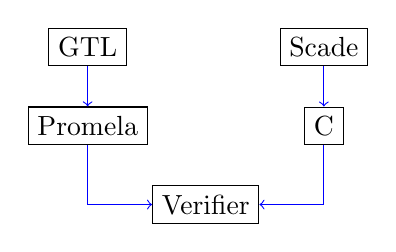
\begin{tikzpicture}
    \node[draw] (gtl) at (0,2) {GTL};
    \node[draw] (scade) at (3,2) {Scade};
    \node[draw] (promela) at (0,1) {Promela};
    \node[draw] (c) at (3,1) {C};
    \node[draw] (verifier) at (1.5,0) {Verifier};
    \draw[->,blue] (gtl) -- (promela);
    \draw[->,blue] (scade) -- (c);
    \draw[->,blue] (promela) |- (verifier);
    \draw[->,blue] (c) |- (verifier);
  \end{tikzpicture}
  \caption{Simulation durch C-Integration von Promela}
\end{figure}

Diese Übersetzungsmethode führt keine Optimierungen oder Abstraktionen durch, sondern simuliert das Modell exakt so, wie durch die Spezifikation angegeben.
Die Kontrakte für die synchronen Komponenten werden also ignoriert.

Zunächst wird jede synchrone Komponente mit Hilfe des SCADE-Compilers nach C übersetzt.
Da der Übersetzungsprozess für jede Komponente einzeln durchgeführt werden muss, muss darauf geachtet werden, dass die Modelle keine Namenskonflikte aufweisen oder die gleichen Sub-Komponenten enthalten\cite{scade_c_integration}.

Dabei generiert der Compiler für jede Komponente zwei Datenstrukturen, die eine enthält die Eingabevariablen, die andere die Ausgabevariablen sowie den internen Zustand der Komponente.
Außerdem werden zwei Funktionen erstellt:
Die erste initialisiert den internen Zustand der Komponente, die zweite führt einen einzelnen Berechnungsschritt der Komponente durch.

%Jede synchrone Komponente wird nun durch einen Promela-Prozess repräsentiert, der zunächst die Datenstrukturen initialisiert und dann in jedem Schritt die Eingabevariablen in die C-Datenstruktur kopiert, die Schrittfunktion aufruft und die Ergebnisse in die Ausgabevariablen schreibt.
Die Übersetzung geht nun wie folgt vor:
Zunächst wird für jeden Prozess eine Instanz der Zustands-Datenstruktur zum globalen Zustandsvektor hinzugefügt.
Dies geschieht über die Verwendung des "`c\_state"'-Konstruktes in Promela.
Eine Komponente "`Engine"' würde beispielsweise den folgenden Code generieren:
\begin{lstlisting}[language=promela]
c_state "outC_Engine Engine_state" "Global"
\end{lstlisting}
Dies fügt dem Zustandsvektor die Variable "`Engine\_state"' hinzu.
Das Schlüsselwort "`Global"' führt dazu, dass auf die Variable von jedem Prozess aus zugegriffen werden kann.

Die Eingabe-Datenstruktur der Komponenten ist für den Zustand des Gesamtsystems nicht entscheidend, sondern wird nur benötigt, um die Eingabesignale der Komponente vor dem Berechnungsschritt zu sammeln.
Deswegen ist es ausreichend, die Struktur mit dem "`c\_decl"'-Konstrukt zu deklarieren:
\begin{lstlisting}[language=promela]
c_decl {
  inC_Engine Engine_input;
}
\end{lstlisting}

Zur korrekten Simulation der synchronen Komponente müssen nun folgende Dinge geschehen:
\begin{enumerate}
\item Am Anfang der Simulation muss die Zustands-Datenstruktur der Komponente initialisiert werden.
  Hierfür generiert der Code-Generator eine "`reset"' Funktion:
  \begin{lstlisting}[language=promela]
c_code {
  Engine_reset(&now.Engine_state);
}
  \end{lstlisting}
\item In jedem Berechnungsschritt müssen die Eingaben für die Komponente aus den Aus\-ga\-be-Da\-ten\-struk\-tu\-ren der verbundenen Komponenten kopiert werden.
  \begin{lstlisting}[language=promela]
c_code {
  Engine_input.power = now.Power_state.on;
  Engine_input.mode = now.SpeedRegulator_state.output;
}
  \end{lstlisting}
\item Die generierte Schrittfunktion der Komponente muss aufgerufen werden.
  \begin{lstlisting}[language=promela]
c_code {
  Engine(&Engine_input,&now.Engine_state);
}
  \end{lstlisting}
\end{enumerate}
